% Fichero principal de transparencias (incluye a todos los dem�s).

% Compilar a .pdf con LaTeX (pdflatex)
% Es necesario instalar Beamer (paquete latex-beamer en Debian)
%

% Gr�ficos:
% Los gr�ficos pueden suministrarse en PNG, JPG, TIF, PDF, MPS
% Los EPS deben convertirse a PDF (usar epstopdf)
%


\documentclass{beamer}
\usetheme{Warsaw}
%\usebackgroundtemplate{
\includegraphics[width=\paperwidth]{format/libresoft-bg-soft.png}}
\usepackage[spanish]{babel}
\usepackage[latin1]{inputenc}
\usepackage{graphics}
\usepackage{amssymb} % Simbolos matematicos

%\definecolor{libresoftgreen}{RGB}{162,190,43}
%\definecolor{libresoftblue}{RGB}{0,98,143}

%\setbeamercolor{titlelike}{bg=libresoftgreen}

%% Metadatos del PDF.
\hypersetup{
  pdftitle={M�ster de econom�a digital: �rea TIC},
  pdfauthor={Jes�s M. Gonz�lez Barahona, Gregorio Robles, Felipe Ortega, Miquel Vidal},
  pdfcreator={Universidad Rey Juan Carlos / EOI},
  pdfproducer=PDFLaTeX,
  pdfsubject={},
}
%%

\AtBeginSection[]
{
\begin{frame}<beamer>
\begin{center}
{\Huge \insertsection}
\end{center}
\end{frame}
}

%%%%%%%%%%%%%%%%%%%%%%%%%%%%%%%%%%%%%%%%%%%%%%%%%%%%%%%%%%%%%%%%
%%%%%%%%%%%%%%%%%%%%%%%%%%%%%%%%%%%%%%%%%%%%%%%%%%%%%%%%%%%%%%%%
% include-only                                                 %
%%%%%%%%%%%%%%%%%%%%%%%%%%%%%%%%%%%%%%%%%%%%%%%%%%%%%%%%%%%%%%%%
%%%%%%%%%%%%%%%%%%%%%%%%%%%%%%%%%%%%%%%%%%%%%%%%%%%%%%%%%%%%%%%%
%\includeonly{presentacion}
% \includeonly{motivacion}
%\includeonly{wikipedia}
\includeonly{presentacion-modulo2}
%\includeonly{licencias}
%\includeonly{fundamentos}
%\includeonly{modelos-negocio}
%\includeonly{modelos-negocio_obras_libres}
%\includeonly{modelos-negocio_ejercicio}
%\includeonly{modelos-negocio,modelos-negocio_modelobras_libres,modelos-negocio_ejercicio}

%\includeonly{casos,notas-finales}

\begin{document}

\title{�rea TIC}
\subtitle{Master de Econom�a Digital e Industrias Creativas, EOI}
\author{Jes�s M. Gonz�lez Barahona, Gregorio Robles, Felipe Ortega}
\institute{{jgb,grex,jfelipe,mvidal}@gsyc.es \\
Universidad Rey Juan Carlos / EOI}

\date{Mayo 2011}

\frame{
\maketitle
\begin{center}

\includegraphics[width=6cm]{format/gsyc-urjc}
\end{center}
}


% Si el titulo o el autor se quieren acortar para los pies de p�gina
% se pueden redefinir aqu�:
%\title{Titulo corto}
%\author{Autores abreviado}


%% LICENCIA DE REDISTRIBUCION DE LAS TRANSPAS
\frame{
~
\vspace{4cm}

\begin{flushright}
\copyright 2002-2011 Jes�s M. Gonz�lez Barahona, Gregorio Robles, Felipe Ortega. Miquel Vidal \\

Algunos derechos reservados. Este art�culo se distribuye bajo
la licencia ``Reconocimiento-CompartirIgual 3.0 Espa�a'' de Creative Commons,
disponible en \url{http://creativecommons.org/licenses/by-sa/3.0/es/deed.es}

Este documento (o uno muy similar) est� disponible en \\
\url{http://gsyc.es}
\end{flushright}
}
%%

%%%%%%%%%%%%%%%%%%%%%%%%%%%%%%%%%%%%%%%%%%%%%%%%%%%%%%%%%%%%%%%%
%%%%%%%%%%%%%%%%%%%%%%%%%%%%%%%%%%%%%%%%%%%%%%%%%%%%%%%%%%%%%%%%
% lista de temas                                               %
%%%%%%%%%%%%%%%%%%%%%%%%%%%%%%%%%%%%%%%%%%%%%%%%%%%%%%%%%%%%%%%%
%%%%%%%%%%%%%%%%%%%%%%%%%%%%%%%%%%%%%%%%%%%%%%%%%%%%%%%%%%%%%%%%
%\documentclass{beamer}
% imprimir
% \documentclass[handout]{beamer} 
% \usepackage{pgfpages}
% \pgfpagesuselayout{4 on 1}[a4paper,landscape,border shrink=5mm]

\mode<presentation> {
  \usetheme{Warsaw}
  \setbeamercovered{transparent}
}

\usebackgroundtemplate{
\includegraphics[width=\paperwidth]{format/libresoft-bg.png}}
\usepackage[spanish]{babel}
\usepackage[utf8]{inputenc}
\usepackage{graphics}
\usepackage{amssymb} % Simbolos matematicos

%\definecolor{libresoftgreen}{RGB}{162,190,43}
%\definecolor{libresoftblue}{RGB}{0,98,143}

%\setbeamercolor{titlelike}{bg=libresoftgreen}

%% Metadatos del PDF.
\hypersetup{  
  pdftitle={Presentación del curso},
  pdfauthor={Miguel Vidal, Jose Castro},
  pdfcreator={GSyC/Libresoft},
  pdfproducer=PDFLaTeX,
  pdfsubject={Arquitectura de servidores con software libre},
}
%%

\begin{document}

\title{Presentación del curso}
\subtitle{Arquitectura de servidores con software libre}
\institute{\{mvidal,jfcastro\}@libresoft.es} 
\author{Miguel Vidal, Jose Castro}
\date{25 de marzo de 2011}

\frame{
\maketitle
\begin{center}

\includegraphics[width=6cm]{format/gsyc-urjc}
\end{center}
}

\frame{
~
\vspace{4cm}

\begin{flushright}
{\small
(cc) 2009-2011 Miguel Vidal, Jose Castro. \\
  Esta presentación se publica bajo una licencia Creative Commons Reconocimiento 3.0 España, disponible en 
  \url{http://creativecommons.org/licenses/by/3.0/es/}
 

\bigskip

}
\end{flushright}
}
%%

\section{Introducción}

\begin{frame}
\frametitle{Información general}
\textbf{Objetivo}\\
Ofrecer una panorámica de las soluciones que ofrece el software libre para construir complejas arquitecturas virtualizadas.\\
\textbf{Fechas}\\
Inicio: 25 de marzo 2011 -- Fin: 10 de junio 2011\\
\textbf{Horario}\\
Viernes de 16:30h a 20:30h\\
\textbf{Lugar}\\
Madrid On Rails\\
\textbf{Material}\\
Ordenador y libro de referencia\\
\textbf{Título}\\
Título propio de la URJC.\\
Al finalizar se obtendrá el certificado de aprovechamiento del curso.
\end{frame}

\section{Temario}
\begin{frame}
\frametitle{Clases}
\begin{enumerate}
\item \textbf{Introduccion}
\item \textbf{Seguridad}
\item \textbf{Sistemas operativos libres}
\item \textbf{Redes}
\item \textbf{Storage as a Service (StaaS)}
\item \textbf{Servicios de Internet}
\item \textbf{Virtualización I}
\item \textbf{Virtualización II}
\item \textbf{Cloud Computing}
\item \textbf{Clusters de Alta Disponibilidad}
\end{enumerate}
\end{frame}

\begin{frame}
  \frametitle{Introducción}
  \textbf{Fecha}\\
    25 de marzo\\
  \textbf{Conferencia}
    \begin{itemize}
      \item \textit{Invitado:} Gregorio Robles -- Director del curso
      \item \textit{Conferencia:} Introducción al software libre
    \end{itemize}
  \textbf{Sesión}
    \begin{itemize}
      \item Metodología del curso
      \item \textit{Profesores:} Jose Castro
    \end{itemize}
    \begin{itemize}
      \item Introducción a la administración de sistemas
      \item \textit{Profesores:} Miguel Vidal
    \end{itemize}
\end{frame}

\begin{frame}
  \frametitle{Seguridad}
  \textbf{Fecha}\\
    1 de abril\\
  \textbf{Conferencia}
    \begin{itemize}
      \item \textit{Invitado:} Eva Castro -- Ph.D. URJC
      \item \textit{Conferencia:} IPv6
    \end{itemize}
  \textbf{Sesión}
    \begin{itemize}
      \item Seguridad proactiva
      \item \textit{Profesores:} Pedro Coca 
    \end{itemize}
    \begin{itemize}
      \item Criptografía de clave pública
      \item \textit{Profesor:} Israel Herráiz -- Ph.D. UCM
    \end{itemize}
\end{frame}

\begin{frame}
  \frametitle{Sistemas operativos libres}
  \textbf{Fecha}\\
    8 de abril\\
  \textbf{Conferencia}
    \begin{itemize}
      \item \textit{Invitado:} David Villanueva -- Ártica
      \item \textit{Conferencia:} Monitorización con Pandora
    \end{itemize}
  \textbf{Sesión}
    \begin{itemize}
      \item Sistemas operativos libres
      \item \textit{Profesores:} Miguel Vidal, Jose Castro
    \end{itemize}
\end{frame}

\begin{frame}
  \frametitle{Redes}
  \textbf{Fecha}\\
    29 de abril\\
  \textbf{Conferencia}
    \begin{itemize}
      \item \textit{Invitado:} Juan José Amor -- Notario de CACert
      \item \textit{Conferencia:} Certificación con CACert
    \end{itemize}
  \textbf{Sesión}
    \begin{itemize}
      \item Redes
      \item \textit{Profesores:} Miguel Vidal, Jose Castro
    \end{itemize}
\end{frame}

\begin{frame}
  \frametitle{Storage as a Service}
  \textbf{Fecha}\\
    6 de Mayo\\
  \textbf{Conferencia}
    \begin{itemize}
      \item \textit{Invitado:} Javier Turégano -- Ándago
      \item \textit{Conferencia:} La experiencia con software libre en empresas TIC
    \end{itemize}
  \textbf{Sesión}
    \begin{itemize}
      \item Storage as a Service
      \item \textit{Profesores:} Miguel Vidal, Jose Castro
    \end{itemize}
\end{frame}

\begin{frame}
  \frametitle{Servicios de Internet}
  \textbf{Fecha}\\
    13 de mayo\\
  \textbf{Conferencia}
    \begin{itemize}
      \item \textit{Invitado:} Álvaro Lopez Ortega -- Líder del proyecto Cherokee
      \item \textit{Conferencia:} Servidor Web Cherokee
    \end{itemize}
  \textbf{Sesión}
    \begin{itemize}
      \item Servicios de Internet
      \item \textit{Profesores:} Miguel Vida, Jose Castro
    \end{itemize}
\end{frame}

\begin{frame}
  \frametitle{Virtualización I}
  \textbf{Fecha}\\
    20 de mayo\\
  \textbf{Conferencia}
    \begin{itemize}
      \item \textit{Invitado:} Víctor Fernández -- SIA Group
      \item \textit{Conferencia:} Evolución del CPD, convergencia de almacenamiento y virtualización
    \end{itemize}
  \textbf{Sesión}
    \begin{itemize}
      \item Virtualización I
      \item \textit{Profesores:} Miguel Vidal, Jose Castro
    \end{itemize}
\end{frame}

\begin{frame}
  \frametitle{Virtualización II}
  \textbf{Fecha}\\
    27 de mayo\\
  \textbf{Conferencia}
    \begin{itemize}
      \item \textit{Invitado:} Juan José Amor -- OpenSistemas \& Gnome Hispano
      \item \textit{Conferencia:} Virtualización en SPARC con LDOMs
    \end{itemize}
  \textbf{Sesión}
    \begin{itemize}
      \item Virtualización II
      \item \textit{Profesores:} Miguel Vidal, Jose Castro
    \end{itemize}
    \begin{itemize}
      \item De la virtualización al Cloud Computing
      \item \textit{Profesores:} Pedro Coca
    \end{itemize}
\end{frame}

\begin{frame}
  \frametitle{Cloud Computing}
  \textbf{Fecha}\\
    3 de junio\\
  \textbf{Conferencia}
    \begin{itemize}
      \item \textit{Invitado:} Constantino Vázquez -- Equipo de desarrollo OpenNebula
      \item \textit{Conferencia:} OpenNebula
    \end{itemize}
  \textbf{Sesión}
    \begin{itemize}
      \item Tutorial de OpenNebula
      \item \textit{Profesores:} Constantino Vázquez
    \end{itemize}
\end{frame}

\begin{frame}
  \frametitle{Alta disponibilidad}
  \textbf{Fecha}\\
    10 de junio\\
  \textbf{Conferencia}
    \begin{itemize}
      \item \textit{Invitado:} Departamento jurídico de Google
      \item \textit{Conferencia:} Aspectos legales del Cloud Computing
    \end{itemize}
  \textbf{Sesión}
    \begin{itemize}
      \item Clusters de alta disponibilidad
      \item \textit{Profesores:} Miguel Vidal, Jose Castro
    \end{itemize}
\end{frame}


\section{Metodología}
\begin{frame}
  \frametitle{Metodología}
  \begin{center}
    \textbf{Moodle} -- \url{http://moodle.libresoft.es}
  \end{center}
  \begin{itemize}
    \item Material del curso: transpas, referencias...
    \item Ejercicios
    \item Foro de dudas
    \item Noticias y avisos
  \end{itemize}
  \vspace{0.15cm}
  \begin{center}
    \textbf{Syllabus}\\
  \end{center}
  \begin{itemize}
    \item Se irá completando durante el curso
    \item Información más completa de las sesiones
    \item Ejercicios y prácticas
  \end{itemize}
\end{frame}

\begin{frame}
  \frametitle{Clases}
  La estructura de las clases será la siguiente:
  \begin{itemize}
    \item Test previo de autoevaluación (no evaluable)
    \item Conferencia de un profesional -- 1 hora
    \item Resolución de ejercicios propuestos -- 30 minutos
    \item Descanso -- 15 minutos
    \item Sesión teórica -- 2 horas y 15 minutos
    \item Ejercicios y prácticas durante la semana -- no más de 1 hora
  \end{itemize}
\end{frame}

\begin{frame}
  \frametitle{Equipos y material}
  \begin{itemize}
    \item Puedes traer tu propio portátil
    \item WIFI para el entorno:
      \begin{itemize}
        \item ESSID:   
        \item usuario: 
        \item contraseña: 
      \end{itemize}
    \item HashTag Twitter: \#casul (Curso Arq. Sistemas Urjc Libresoft)
    \item Canal IRC: \textit{\#casul} en irc.freenode.net
  \end{itemize}
\end{frame}

\begin{frame}
  \frametitle{Evaluación}
  \begin{itemize}
    \item Ejercicios Moodle -- 40\%
    \item Práctica final -- 60\%
    \item Entradas en el blog -- 10\% \textit{(opcional)}
    \item Participación
  \end{itemize}
\end{frame}


\section{Contacto}
\begin{frame}
  \frametitle{Contacto}
  \begin{itemize}
    \item E-mail: \{mvidal,jfcastro\}@libresoft.es
    \item Twitter: @mvidallopez y @jfcastroluis
    \item Moodle: \url{http://moodle.libresoft.es}
    \item Canal de IRC: \textit{\#casul} en irc.freenode.net
  \end{itemize}
\end{frame}

\begin{frame}
  \frametitle{Preguntas}
  \begin{center}
    \huge{Preguntas y dudas}
  \end{center}
\end{frame}

\begin{frame}
  \frametitle{Presentación}
  \begin{center}
    \huge{Os toca presentaros}
  \end{center}
\end{frame}

% Fin del documento
\end{document}

%%---------------------------------------------------------------
%%---------------------------------------------------------------
\section{Motivaci�n}

\begin{frame}
\frametitle{�Pirater�a?}

\vspace{1cm}

\begin{quotation}
``Si t� tienes una manzana, yo tengo una manzana y las
intercambiamos, seguiremos teniendo una manzana
cada uno. Pero si t� tienes una idea, yo tengo una idea, y las
intercambiamos, cada uno de nosotros tendr� dos ideas.''
\end{quotation}

\begin{flushright}
Atribuido a Bernard Shaw
\end{flushright}
\end{frame}

%%---------------------------------------------------------------

\begin{frame}
\frametitle{�Plagio?}

\vspace{1cm}

\begin{quotation}
``Si he visto m�s lejos es porque me sub� en hombros de gigantes''
\end{quotation}

\begin{flushright}
Isaac Newton \\
Carta a Robert Hooke, 15 de febrero de 1676
\end{flushright}
\end{frame}

%%---------------------------------------------------------------

\begin{frame}

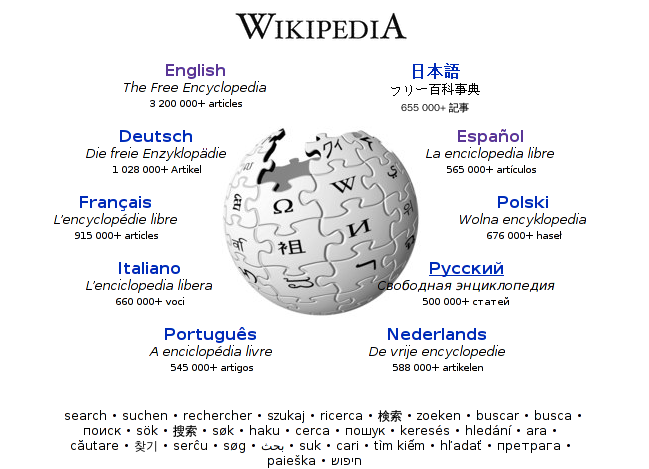
\includegraphics[height=7.5cm]{wikipedia}

\end{frame}

%%---------------------------------------------------------------

\begin{frame}

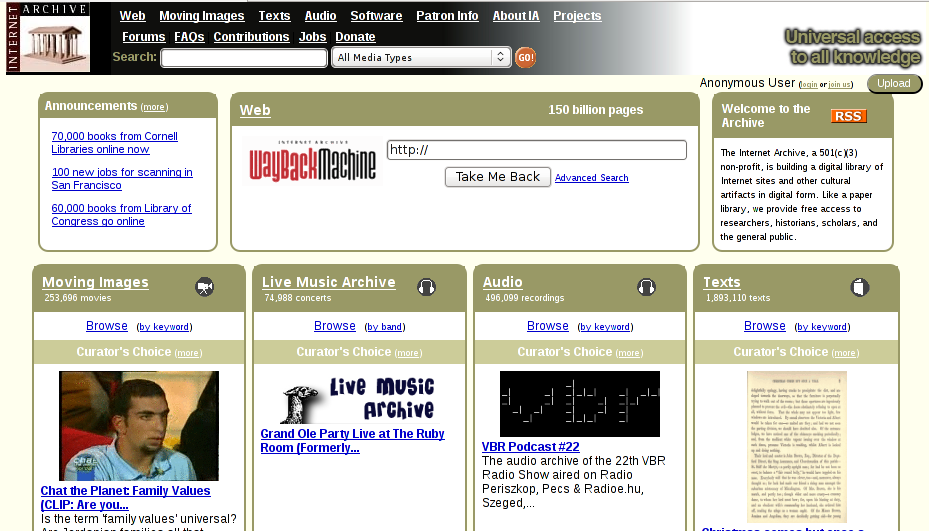
\includegraphics[height=6.5cm]{internet-archive}
\begin{flushright}
\url{http://www.archive.org/}
\end{flushright}
\end{frame}

%%---------------------------------------------------------------

\begin{frame}

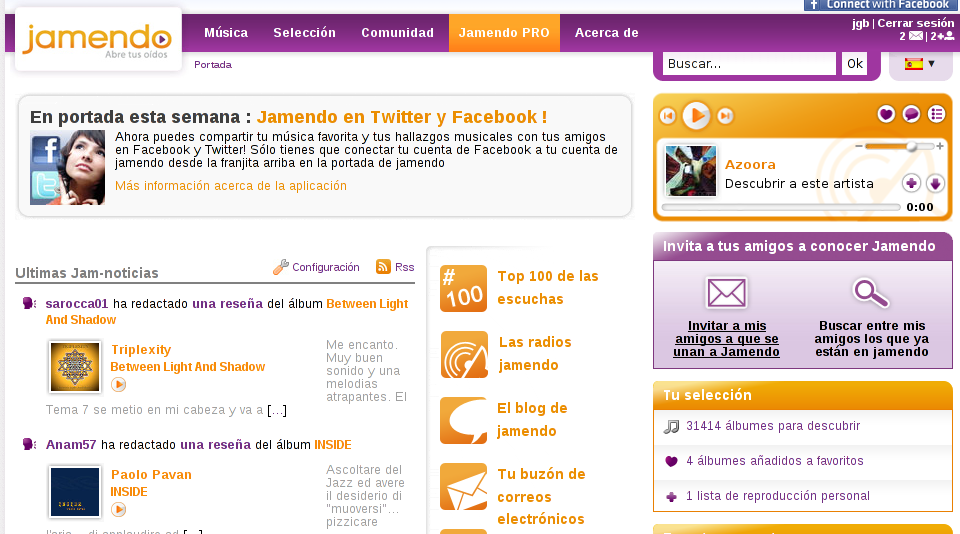
\includegraphics[height=6.5cm]{jamendo}
\begin{flushright}
\url{http://www.jamendo.com/es/}
\end{flushright}
\end{frame}

%%---------------------------------------------------------------

\begin{frame}

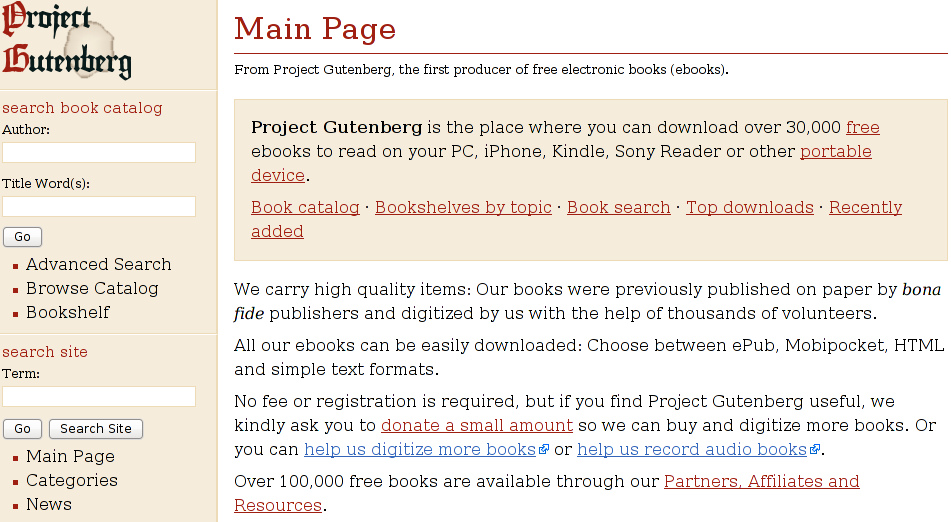
\includegraphics[height=6cm]{gutenberg}
\begin{flushright}
\url{http://www.gutenberg.org}
\end{flushright}
\end{frame}

%%---------------------------------------------------------------

\begin{frame}
\frametitle{Una (antigua) utop�a hecha realidad...}

Con las obras que son informaci�n, podemos:

\begin{itemize}
\item copiarlas
\item transportarlas a casi cualquier lugar del mundo
\item crear modificaciones
\end{itemize}

Todo ello con gran facilidad, casi sin coste, en grandes cantidades,
para grandes p�blicos potenciales...

...y por primera vez desde que sabemos crear esas obras.

\end{frame}

%%---------------------------------------------------------------

\begin{frame}
\frametitle{�Qu� hacemos con ella?}

\begin{itemize}
\item Por ahora no mucho...
\item ...quiz�s, lo mismo de siempre, pero m�s r�pido, m�s barato
\item Algunos experimentos est�n mostrando nuevas posibilidades...
\item ...pero a veces los asfixiamos antes de que muestren sus posibilidades
\end{itemize}

Las posibilidades del siglo XXI se ven limitadas por el entorno
social, econ�mico y jur�dico del XIX.
\end{frame}

%%---------------------------------------------------------------

\begin{frame}
\frametitle{Recordando los or�genes...}

\begin{itemize}
\item ...y al principio no hab�a ``derechos'' de autor
\item Con la imprenta aparecieron... \\
  los derechos del editor
\item Poco a poco los autores tuvimos nuestra parte...
\item ...pero s�lo como fruto de un acuerdo social:
\begin{quote}
La sociedad renuncia a parte de su derecho a la copia \\
(que dif�cilmente podr�a ejercer) \\
a cambio de incentivar la creaci�n de obra intelectual
\end{quote}
\item Pero no lo olvidemos, los monopolios causan distorsiones...
\item ...y hoy la tecnolog�a nos permite ejercer el derecho de copia
\end{itemize}

\end{frame}

%%---------------------------------------------------------------

\begin{frame}
\frametitle{Lo que tarda en cambiar la forma de ver el mundo}

\begin{itemize}
\item Nuevas formas de entender la obra colectiva \\
  Ej: �reelaboraci�n secuencial o plagio?
\item Nuevas formas de entender la distribuci�n \\
  ``Por favor, copiad mis canciones''
\item Los ``consumidores'' se hacen ``productores'' \\
  Cualquiera puede publicar, cualquiera puede comentar (ej: blogs)
\item Nuevas formas de conseguir calidad \\
  Ej: Wikipedia, software libre
\end{itemize}

\end{frame}

%%---------------------------------------------------------------

\begin{frame}
\frametitle{El software libre como frente de ola}

\begin{itemize}
\item M�s de 20 a�os mostrando nuevas formas de producci�n de
  algo tan complejo como los programa de ordenador
\item Alta calidad (al menos, en ciertos casos)
\item Enormes comunidades creadas alrededor de �l
\item Poco a poco influyendo otros campos
\item Mucha experiencia en tratar con los nuevos problemas que aparecen
\end{itemize}

\end{frame}

%%---------------------------------------------------------------

\begin{frame}
\frametitle{�D�nde quedan los derechos digitales en todo esto?}

\begin{itemize}
\item Necesitan redefinici�n
\item Importante no fijar legislaci�n restrictiva antes de conocer en
  detalle los nuevos modelos...
\item ...modelos que a�n estamos empezando a explorar
\item Desde luego, no es posible una simple ``extensi�n'' a las nuevas
  posibilidades tecnol�gicas
\item La tecnolog�a puede limitar tanto (o m�s) que la legislaci�n
\end{itemize}

\end{frame}

%%---------------------------------------------------------------

\begin{frame}
\frametitle{Algunos ejemplos}

\begin{itemize}
\item Nuevo equilibrio entre copia y creaci�n \\
  (ej: Creative Commons)
\item Limitaciones a las tecnolog�as que limitan \\
  (ej: zonificaci�n de DVDs)
\item Margen para experimentar antes de prohibir \\
  (ej: tecnolog�as peer-to-peer)
\item Atenci�n a la gran cantidad de nuevos creadores \\
  (ej: Wikipedia, blogsfera)
\end{itemize}

\end{frame}

%%---------------------------------------------------------------

\begin{frame}
\frametitle{Para terminar...}

\begin{center}
{\LARGE
Estamos ante un mundo nuevo...\\
~ \\
...�lo estamos limitando con ideas viejas?
}
\end{center}

\end{frame}

%%---------------------------------------------------------------
%%---------------------------------------------------------------
\section{Wikipedia: La enciclopedia libre}

%%---------------------------------------------------------------

\subsection{Introducci�n}

%%---------------------------------------------------------------

\begin{frame}
\frametitle{�Qu� es Wikipedia?}

\vspace{1cm}

\begin{center}
{\Large
La enciclopedia libre que todo el mundo puede editar
}
\end{center}

\begin{quotation}
``La promesa de Wikipedia es nada menos que la liberaci�n del conocimiento
humano - tanto por incorporarlo por completo a trav�s del proceso colaborativo,
como por compartirlo libremente con cualquiera que tenga acceso a Internet.
Esta es una idea radicalmente popular.''
\end{quotation}

\begin{flushright}
The Economist, 20 de abril de 2006
\end{flushright}
\end{frame}

%%---------------------------------------------------------------

\begin{frame}
\frametitle{�Qu� es Wikipedia?}

\vspace{1cm}

\begin{center}
{\Large
La enciclopedia libre que todo el mundo puede editar
}
\end{center}

\begin{quotation}
``Wikipedia es lo mejor que hay. Cualquiera en el mundo puede escribir lo que quiera sobre cualquier tema,
as� que sabes que estas obteniendo la mejor informaci�n posible.''
\end{quotation}

\begin{flushright}
Michael Scott (interpretado por Steve Carell) en la serie \textit{The Office} [3.18], 5 de abril de 2007.
\end{flushright}
\end{frame}

%%---------------------------------------------------------------

\begin{frame}
\frametitle{Influencia de Wikipedia: vida diaria}

\vspace{1cm}

\begin{quotation}
``Wikipedia se ha cargado las tertulias de bar. Antes la gente apostaba o discut�a por ver qui�n sab�a m�s
sobre un tema. Ahora alguien saca un m�vil, lo mira en Wikipedia y se acab�.''
\end{quotation}

\begin{flushright}
Intervenci�n de un oyente durante una entrevista sobre los 10 a�os de Wikipedia en \textit{La Ventana, Cadena SER}, 14 de enero de 2011.
\end{flushright}
\end{frame}

%%---------------------------------------------------------------

\begin{frame}
\frametitle{Influencia de Wikipedia: vida diaria}

\vspace{0.5cm}

\begin{quotation}
`` Wikipedia ya no era un mero proyecto secundario curioso y la
ni�a bonita de la �lite tecnol�gica. Ahora estaba en las grandes ligas. La gente
depend�a de ella cada d�a. Una entrada completamente err�nea pod�a ensombrecer miles
de otras fant�sticas, y afectaba la reputaci�n de la gente y la forma en que se ganan la vida''.
\end{quotation}

\begin{flushright}
Andrew Lih, \textit{The Wikipedia Revolution}. \\
Ed. Hyperion, 17 de marzo de 2009.
\end{flushright}
\end{frame}

%%---------------------------------------------------------------

\begin{frame}
\frametitle{Influencia de Wikipedia: vida diaria}

\begin{center}
{\LARGE
Video: Wikipedia entre las 10 p�ginas m�s consultadas por los espa�oles}
\end{center}

%% http://www.rtve.es/alacarta/videos/telediario/wikipedia-esta-entre-diez-paginas-mas-consultadas-espanoles/1107183/

\begin{flushright}
RTVE, 20 de mayo de 2011.
\end{flushright}
\end{frame}

%%---------------------------------------------------------------

\begin{frame}
\frametitle{Influencia de Wikipedia: fiabilidad de los datos}

\vspace{1cm}

\begin{quotation}
``No deber�amos estar us�ndola [Wikipedia] para comprobar ninguna informaci�n que salga en el peri�dico''.
\end{quotation}

\begin{flushright}
Larry Ingrassia, editor de area de negocios en \textit{The New York Times}, tras el ``incidente Seigenthaler'', 12 de julio de 2005.
\end{flushright}
\end{frame}

%%---------------------------------------------------------------

\begin{frame}
\frametitle{Influencia de Wikipedia: fiabilidad de los datos}

\begin{center}
{\LARGE
Video: �Por qu� se colabora de forma altruista en Wikipedia?}
\end{center}

%% http://www.rtve.es/noticias/20110114/por-que-colabora-forma-altruista-wikipedia/395080.shtml

\begin{flushright}
RTVE, 15 de enero de 2011.
\end{flushright}
\end{frame}

%%---------------------------------------------------------------

\begin{frame}

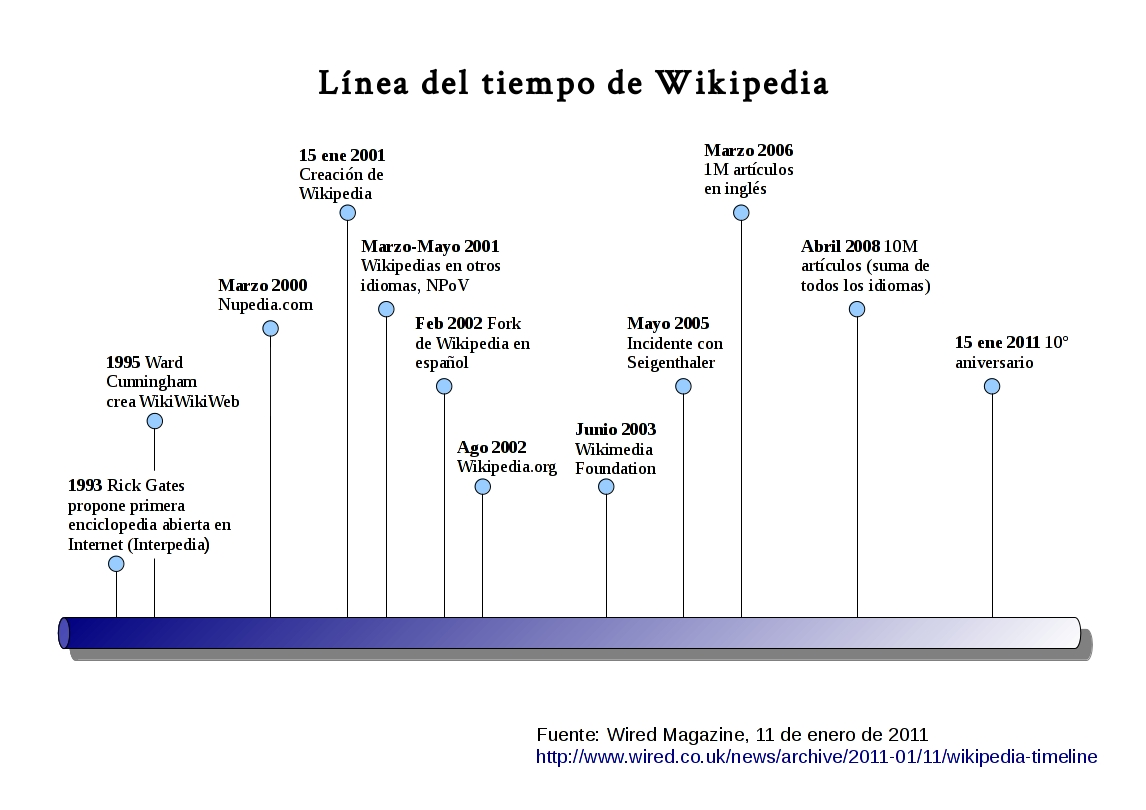
\includegraphics[height = 8cm]{figs/Wikipedia-timeline}

\end{frame}

%%---------------------------------------------------------------
%%---------------------------------------------------------------

\subsection{Trivial sobre Wikipedia}

%%---------------------------------------------------------------

\begin{frame}
\frametitle{Preguntas (y respuestas)}

\begin{itemize}

\item �En cuantos idiomas diferentes est� disponible Wikipedia?
\pause
\begin{itemize}
 \item 278 idiomas diferentes.
\end{itemize}
\pause

\item �Cuantos idiomas en Wikipedia han superado los 300K art�culos?
\pause
\begin{itemize}
 \item 13 idiomas
\end{itemize}
\pause

\item �Y cuantos han superado el mill�n de art�culos?
\pause
\begin{itemize}
 \item 3 idiomas (ingl�s, alem�n y franc�s).
\end{itemize}

\end{itemize}

\end{frame}

%%---------------------------------------------------------------

\begin{frame}
\frametitle{Preguntas (y respuestas)}

\begin{itemize}

\item �Cuantos editores diferentes (con cuenta de usuario) han editado Wikipedia en ingl�s hasta ahora?
\pause
\begin{itemize}
 \item 4.038M de editores.
\end{itemize}
\pause

\item �Cuantas ediciones (en total) ha registrado Wikipedia en ingl�s hasta diciembre de 2010?
\pause
\begin{itemize}
 \item +375M de ediciones.
\end{itemize}
\pause

\item �Cu�ntas contribuciones ha hecho el editor m�s activo de Wikipedia?
\pause
\begin{itemize}
 \item +678K (Wikipedia:List\_of\_Wikipedians\_by\_number\_of\_edits)
\end{itemize}

\end{itemize}

\end{frame}

%%---------------------------------------------------------------
%%---------------------------------------------------------------

\subsection{Navegando por Wikipedia}

%%---------------------------------------------------------------

\begin{frame}
\frametitle{Un art�culo}

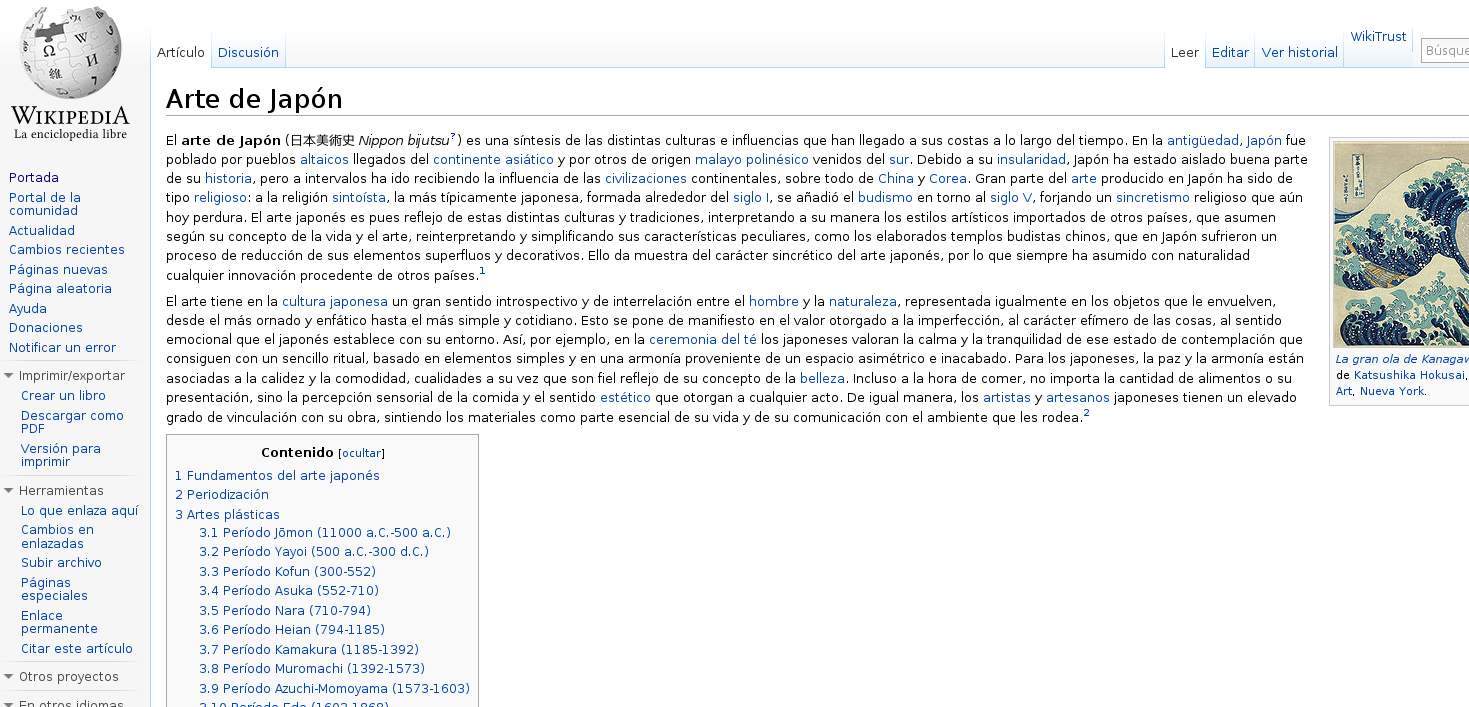
\includegraphics[height=5.5cm]{figs/wikipedia-articulo.png}
\begin{flushright}
Art�culo ``Arte de Jap�n'' en Wikipedia en espa�ol.
\end{flushright}

\end{frame}

%%---------------------------------------------------------------

\begin{frame}
\frametitle{Pesta�as y b�squeda}

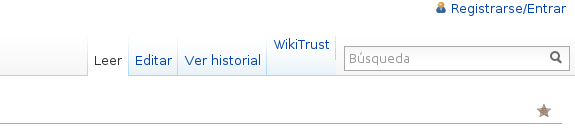
\includegraphics[height=2.5cm]{figs/wikipedia-tabs-search.png}
\begin{flushright}
Detalle de pesta�as y caja de b�squeda de un art�culo.
\end{flushright}

\end{frame}

%%---------------------------------------------------------------

\begin{frame}
\frametitle{Herramientas}

\begin{figure}[htp]
\centering
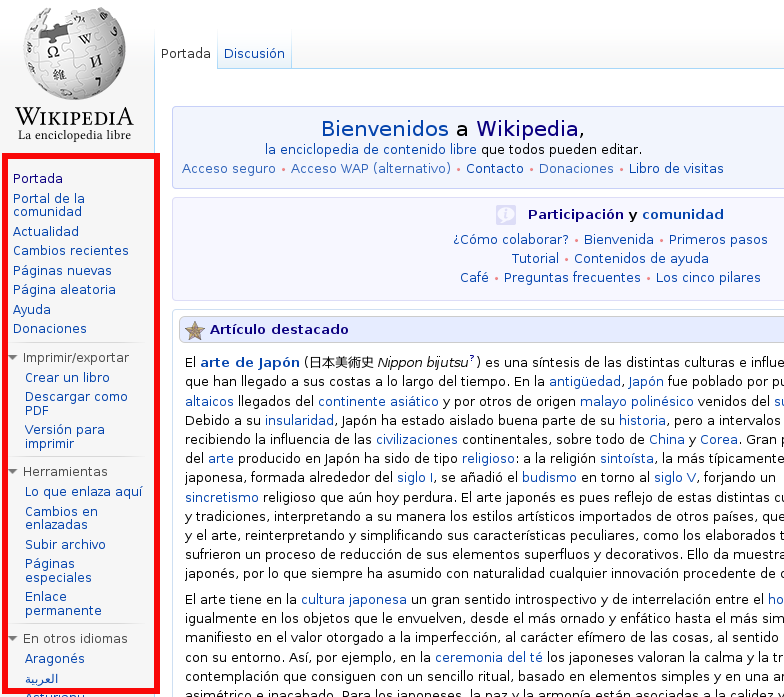
\includegraphics[height=7cm]{figs/wikipedia-toolbox.png}
\end{figure}

\end{frame}

%%---------------------------------------------------------------

\begin{frame}
\frametitle{Enlaces y categor�as}

\begin{itemize}

\item Los art�culos pueden contener enlaces a otras p�ginas de Wikipedia, o de otros sitios de Internet.
\item Tambi�n existen:
\begin{itemize}
 \item V�ase tambi�n.
 \item Referencias.
 \item Bibliograf�a.
 \item Enlaces externos.
\end{itemize}

\item Las categor�as (en una caja al final del art�culo) clasifican las entradas por temas afines.


\end{itemize}

\end{frame}

%%---------------------------------------------------------------

\begin{frame}
\frametitle{Wikiproyectos}

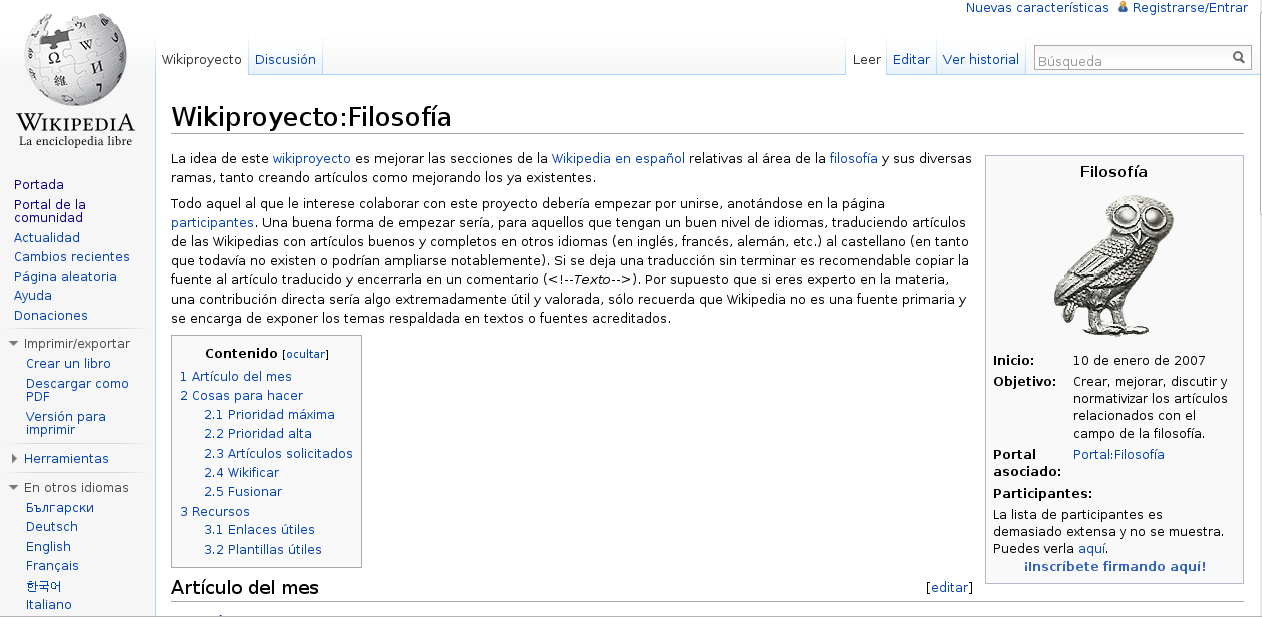
\includegraphics[height=5.5cm]{figs/wikiproyecto-filosofia.png}
\begin{flushright}
{\small\url{http://es.wikipedia.org/wiki/Wikiproyecto:Filosof\%C3\%ADa}}
\end{flushright}

\end{frame}

%%---------------------------------------------------------------

\begin{frame}
\frametitle{Portales}

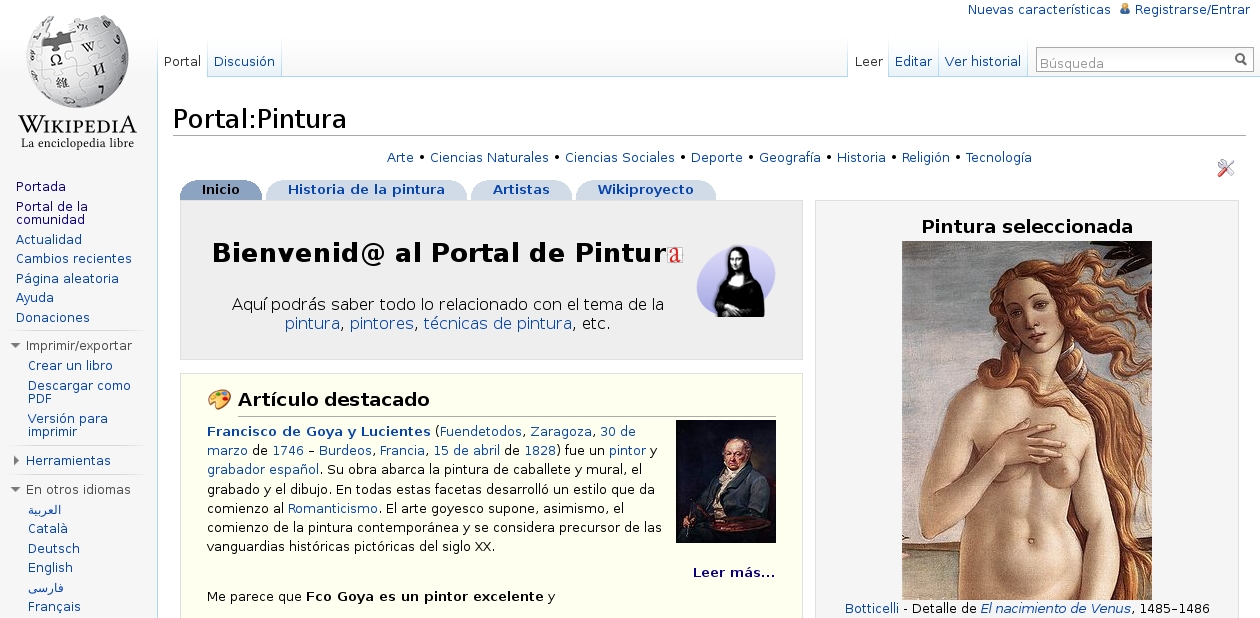
\includegraphics[height=5.5cm]{figs/wikiportal-pintura.png}
\begin{flushright}
\url{http://es.wikipedia.org/wiki/Portal:Pintura}
\end{flushright}

\end{frame}

%%---------------------------------------------------------------

\subsection{Evaluando el contenido de Wikipedia}

%%---------------------------------------------------------------

\begin{frame}
\frametitle{Los 5 pilares de Wikipedia}

\begin{itemize}

\item Es una enciclopedia.
\item Punto de vista neutral.
\item Contenido libre.
\item Normas de etiqueta.
\item No tiene normas fijas.

\end{itemize}

\end{frame}

%%---------------------------------------------------------------

\begin{frame}
\frametitle{Criterios b�sicos: NPoV, NoR y V}

\begin{itemize}

\item NPoV (Punto de Vista Neutral).
\begin{itemize}
 \item Se deben recoger los principales puntos de vista sobre cada tema.
\end{itemize}
\item NoR (No se admite investigaci�n original).
\begin{itemize}
 \item Todo concepto o idea tratado en una enciclopedia debe haber sido publicado y contrastado previamente.
\end{itemize}

\item V (Verificabilidad de la informaci�n aportada).
\begin{itemize}
 \item Todo contenido en Wikipedia debe poder ser contrastado mediante fuentes externas fiables de referencia.
 \item Libros, art�culos, medios de comunicaci�n.
\end{itemize}


\end{itemize}

\end{frame}
%%---------------------------------------------------------------

\subsection{Pr�ctica: C�mo participar en Wikipedia}

%%---------------------------------------------------------------

\begin{frame}
\frametitle{Zona de pruebas}

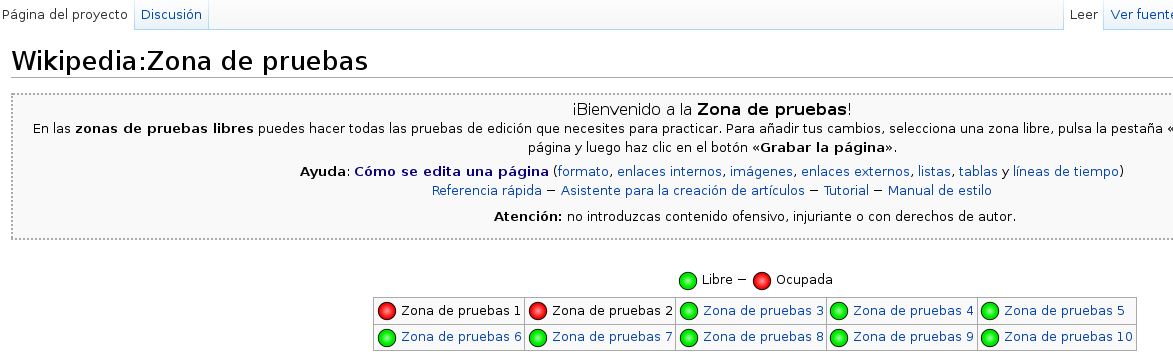
\includegraphics[height=3.5cm]{figs/wikipedia-zona-de-pruebas.png}
\begin{flushright}
{\small\url{http://es.wikipedia.org/wiki/Wikipedia:Zona_de_pruebas}}
\end{flushright}

\end{frame}

%%---------------------------------------------------------------

\begin{frame}
\frametitle{Editar art�culos}

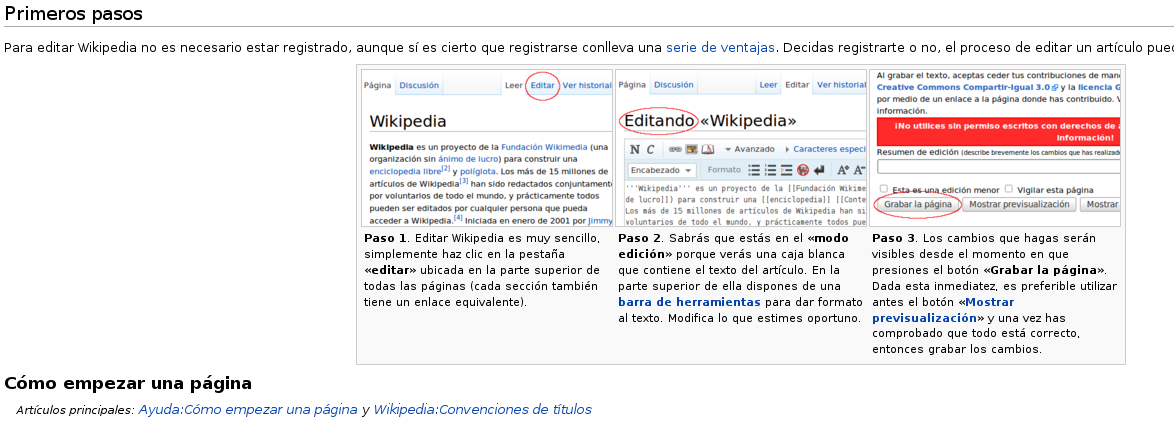
\includegraphics[height=4cm]{figs/wikipedia-primeros-pasos.png}
\begin{flushright}
http://es.wikipedia.org/wiki/Ayuda:C�mo\_se\_edita\_una\_p�gina
\end{flushright}

\end{frame}

%%---------------------------------------------------------------

\begin{frame}
\frametitle{Colaboraci�n: p�ginas de discusi�n}

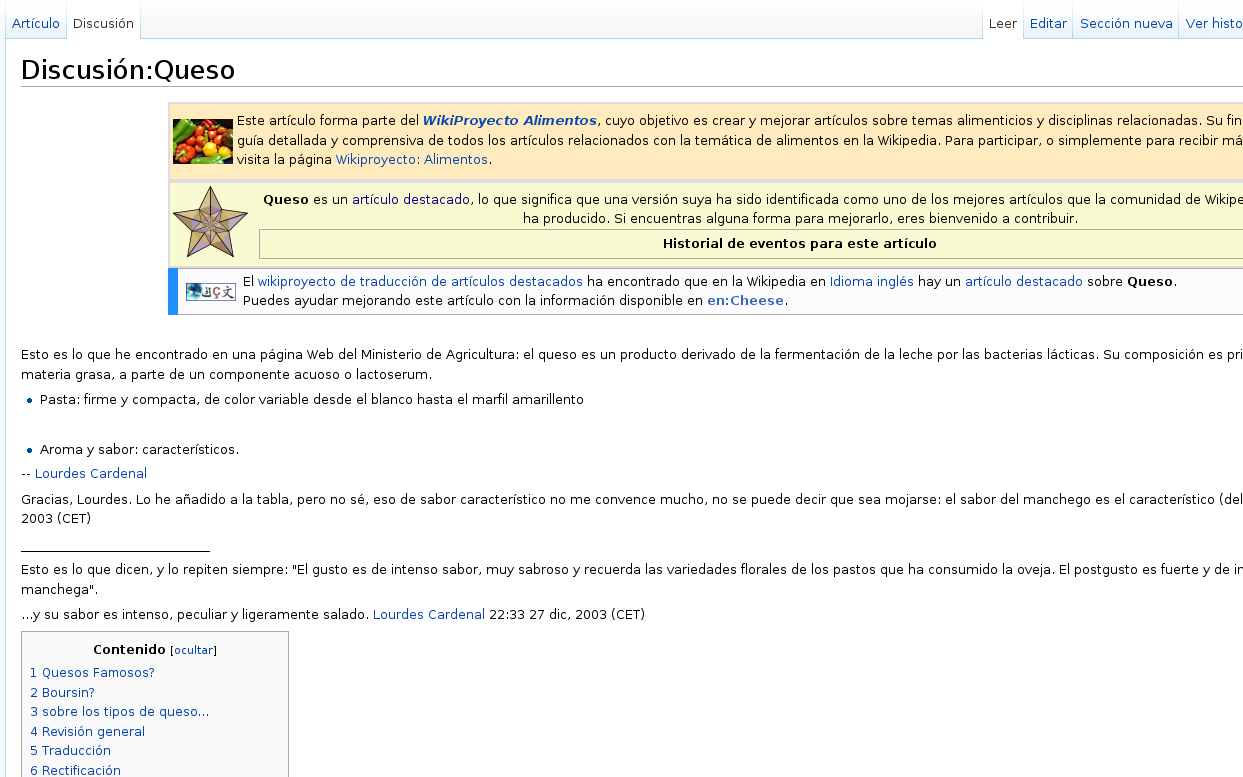
\includegraphics[width=9cm]{figs/wikipedia-talk-page.png}
\begin{flushright}
P�gina de discusi�n del art�culo ``Queso''.
\end{flushright}


\end{frame}

%%---------------------------------------------------------------

\begin{frame}
\frametitle{Im�genes y otros contenidos}

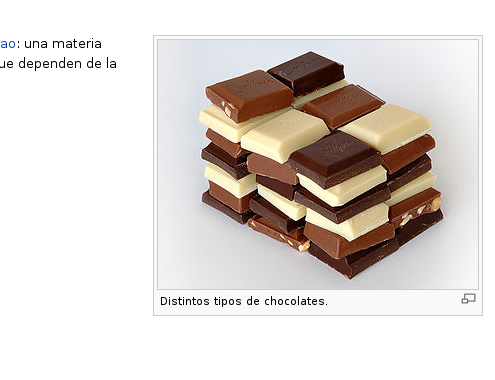
\includegraphics[width=7cm]{figs/wikipedia-imagen.png}
\begin{flushright}
Detalle de una imagen en el art�culo ``Chocolate''.
\end{flushright}

\end{frame}

%%---------------------------------------------------------------

\begin{frame}
\frametitle{Ciclo de vida de los art�culos}

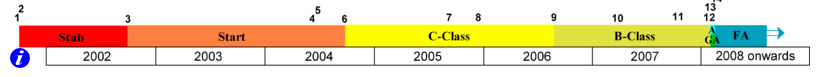
\includegraphics[width=11.5cm]{figs/ciclo-articulo-destacado.png}
\begin{flushright}
Ciclo de vida del art�culo ``Atom'' en ingl�s.
\end{flushright}

\end{frame}

%%---------------------------------------------------------------

\subsection{Comunidad de Wikipedia}

%%---------------------------------------------------------------

\begin{frame}
\frametitle{Wikimania}

\begin{figure}[htp]
\centering
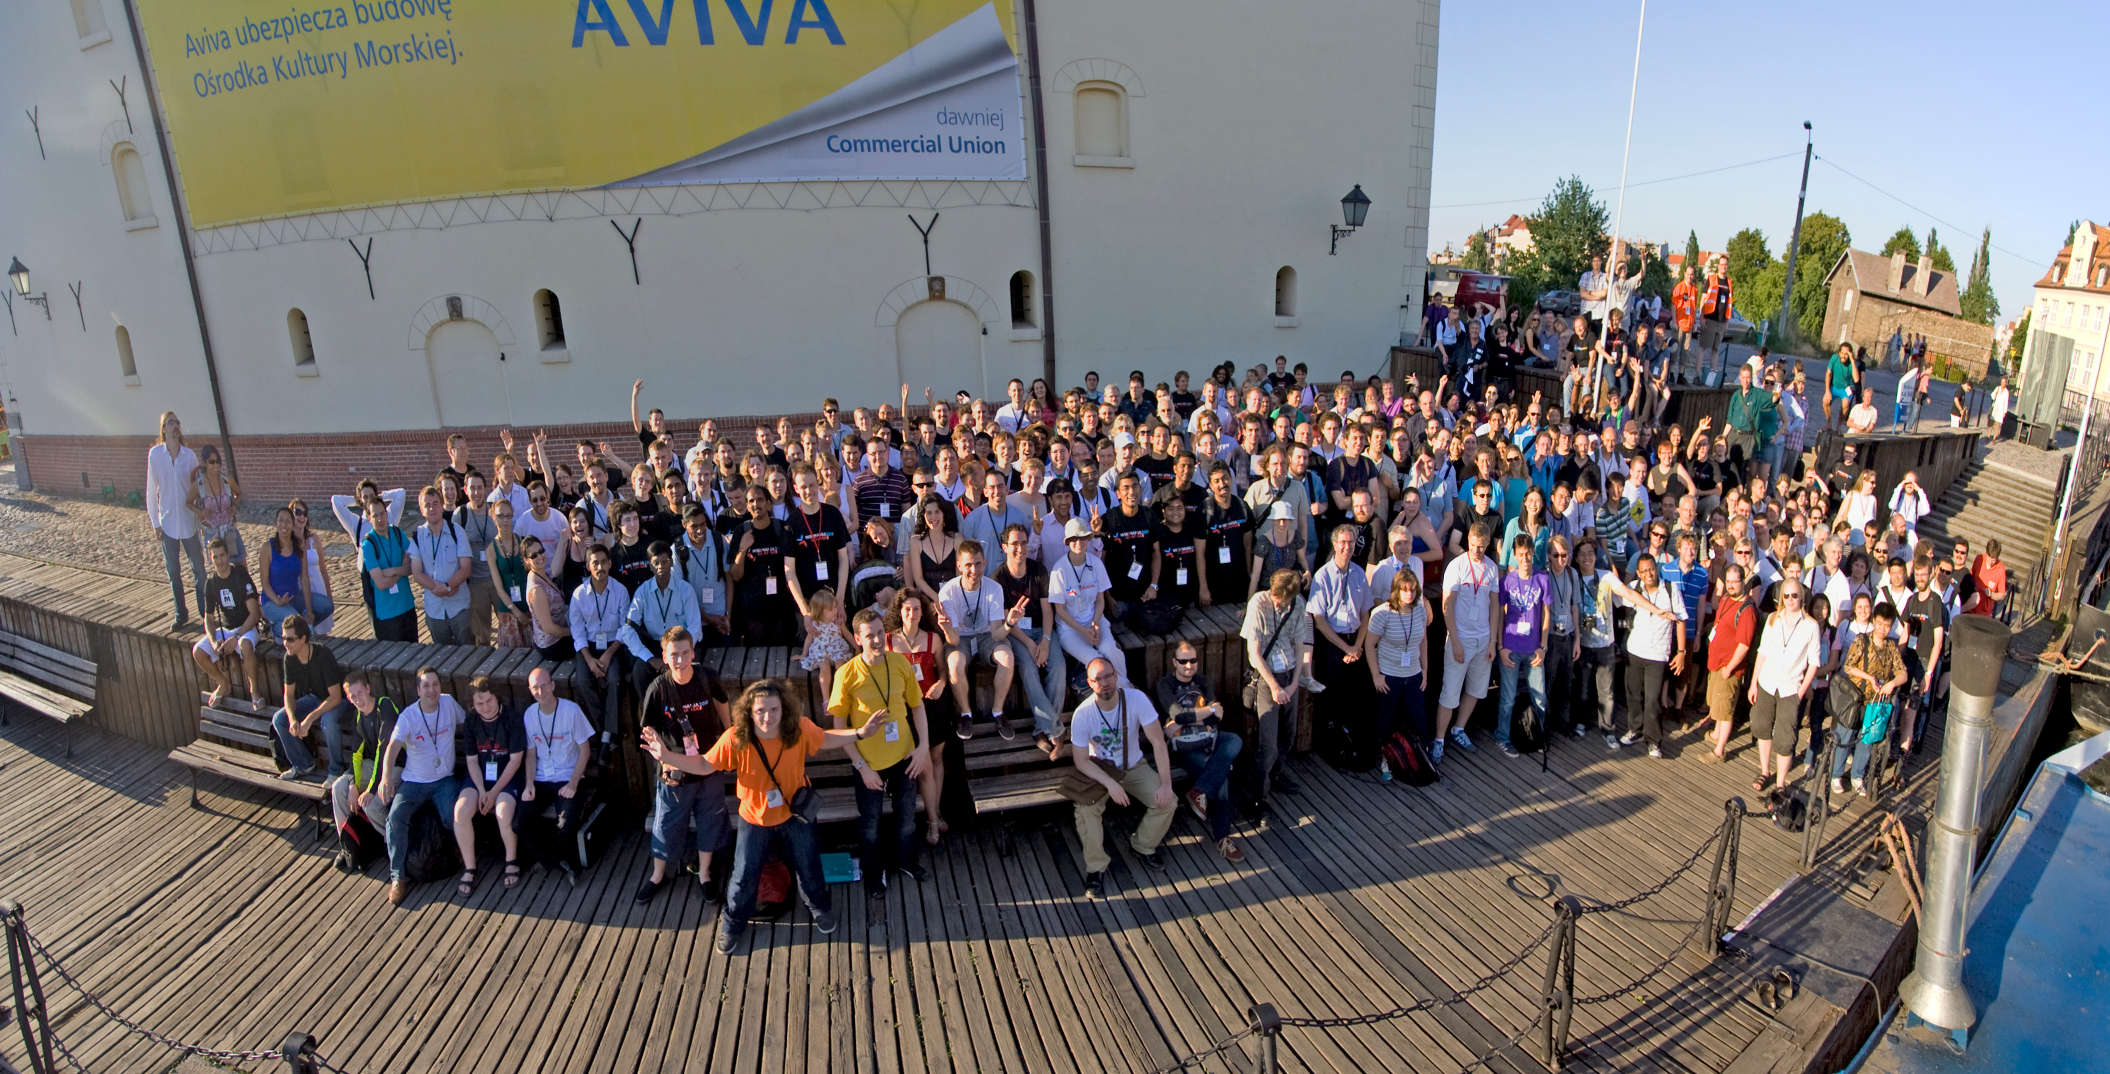
\includegraphics[width=10cm]{figs/wikimania-gdansk-2010.jpg}
\end{figure}

\end{frame}

%%---------------------------------------------------------------

\begin{frame}
\frametitle{Wikimedia Foundation}

\begin{itemize}

\item Fundaci�n sin �nimo de lucro.
\item Creada en 2003.
\item Vela por la sostenibilidad de Wikipedia y otros proyectos asociados.
\item Desarrolla iniciativas a escala global.
\item 31 cap�tulos locales en diferentes pa�ses (inclu�do Espa�a).

\end{itemize}

\end{frame}

%%---------------------------------------------------------------

\begin{frame}
\frametitle{Lo que queda por hacer...}

\begin{itemize}

\item Mejorar la calidad de muchos art�culos.
\item A�adir entradas sobre temas m�s espec�ficos.
\item Ampliar contenidos en bastantes idiomas.
\item Editor m�s intuitivo.
\item Mejorar soporte para contenido no textual.
\item ... inserta aqu� tu propia petici�n.

\end{itemize}

\end{frame}

%%---------------------------------------------------------------
% 
% \begin{frame}
% 
% 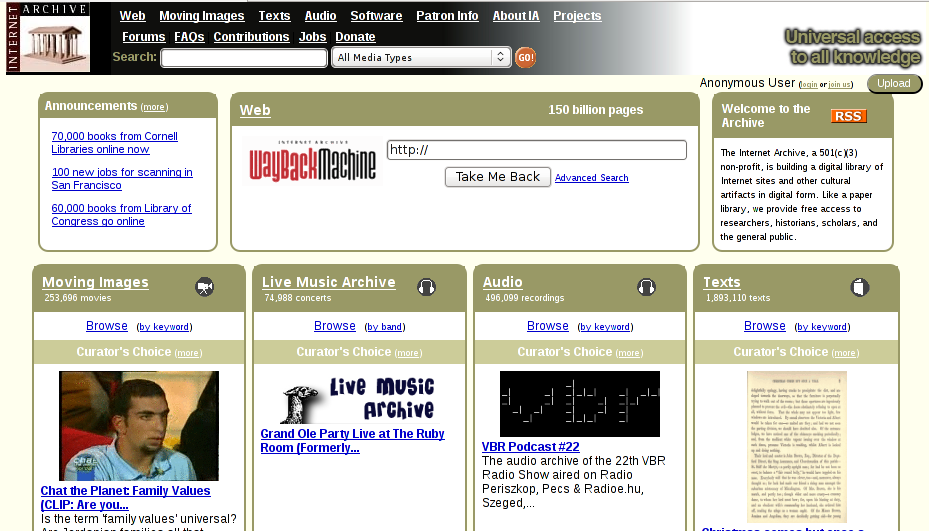
\includegraphics[height=6.5cm]{internet-archive}
% \begin{flushright}
% \url{http://www.archive.org/}
% \end{flushright}
% \end{frame}
% 
% %%---------------------------------------------------------------
% 
% \begin{frame}
% 
% 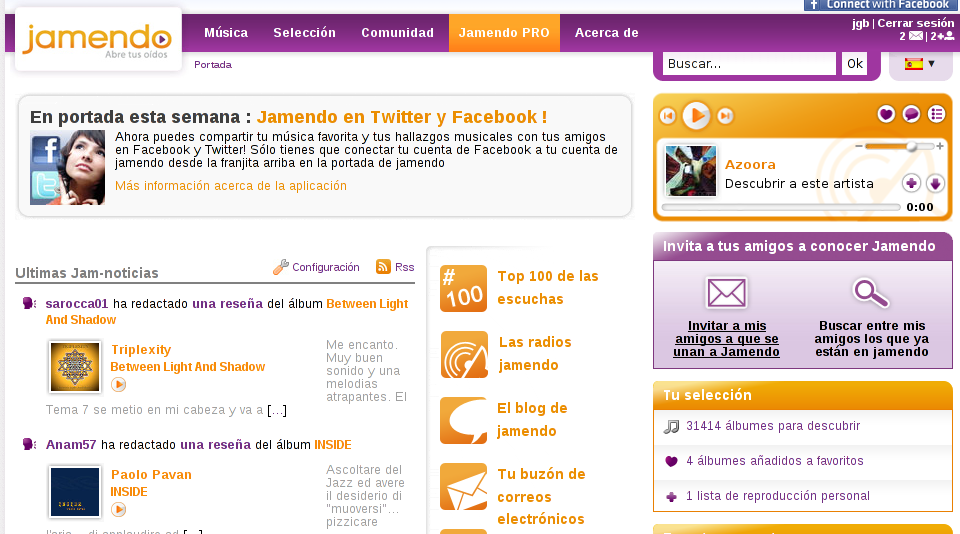
\includegraphics[height=6.5cm]{jamendo}
% \begin{flushright}
% \url{http://www.jamendo.com/es/}
% \end{flushright}
% \end{frame}
% 
% %%---------------------------------------------------------------
% 
% \begin{frame}
% 
% 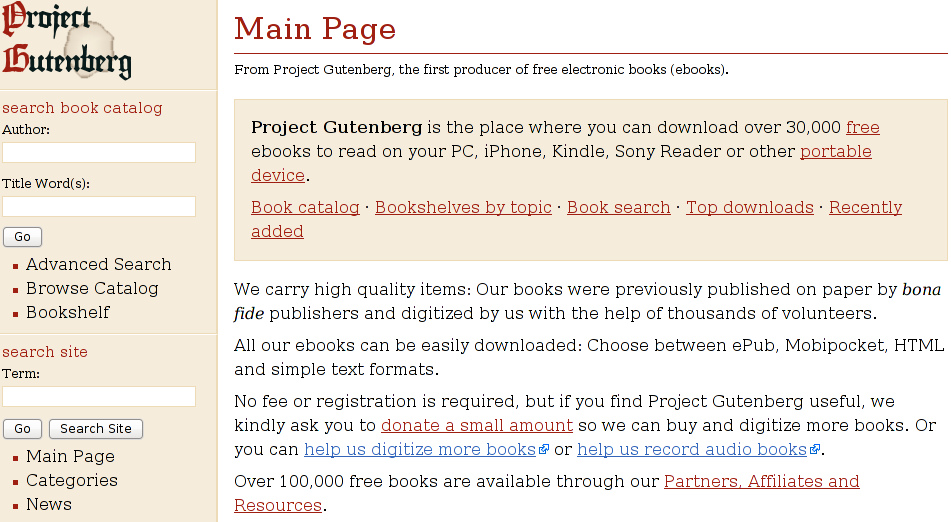
\includegraphics[height=6cm]{gutenberg}
% \begin{flushright}
% \url{http://www.gutenberg.org}
% \end{flushright}
% \end{frame}
% 
% %%---------------------------------------------------------------
% 
% \begin{frame}
% 
% 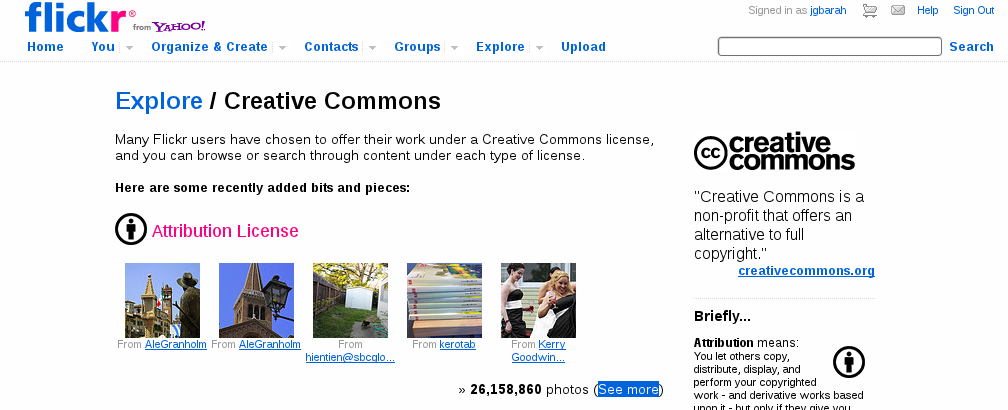
\includegraphics[height=5cm]{flickr-by}
% \begin{flushright}
% \url{http://www.flickr.com/creativecommons/}
% \end{flushright}
% \end{frame}
% 
% %%---------------------------------------------------------------
% 
% \begin{frame}
% \frametitle{Una (antigua) utop�a hecha realidad...}
% 
% Con las obras que son informaci�n, podemos:
% 
% \begin{itemize}
% \item copiarlas
% \item transportarlas a casi cualquier lugar del mundo
% \item crear modificaciones
% \end{itemize}
% 
% Todo ello con gran facilidad, casi sin coste, en grandes cantidades,
% para grandes p�blicos potenciales...
% 
% ...y por primera vez desde que sabemos crearlas.
% 
% \end{frame}
% 
% %%---------------------------------------------------------------
% 
% \begin{frame}
% \frametitle{�Y qu� hacemos?}
% 
% \begin{itemize}
% \item Por ahora no mucho...
% \item Quiz�s lo mismo de siempre, pero m�s r�pido, m�s barato
% \item Algunos experimentos est�n mostrando nuevas posibilidades...
% \item ...pero a veces los asfixiamos antes de que den frutos
% \end{itemize}
% 
% Las posibilidades del siglo XXI se ven limitadas por el entorno
% social, econ�mico, jur�dico y cultural del XIX.
% \end{frame}
% 
% %%---------------------------------------------------------------
% 
% \begin{frame}
% \frametitle{Recordando los or�genes...}
% 
% \begin{itemize}
% \item ...y al principio no hab�a ``derechos'' de autor
% \item Con la imprenta aparecieron... \\
%   los derechos del editor
% \item Poco a poco los autores tuvimos nuestra parte...
% \item ...pero s�lo como fruto de un acuerdo social:
% \begin{quote}
% La sociedad renuncia a parte de su derecho a la copia \\
% (que dif�cilmente podr�a ejercer) \\
% a cambio de incentivar la creaci�n de obra intelectual
% \end{quote}
% \item Pero no lo olvidemos, los monopolios causan distorsiones...
% \item ...y hoy la tecnolog�a nos permite ejercer el derecho de copia
% \end{itemize}
% 
% \end{frame}
% 
% %%---------------------------------------------------------------
% 
% \begin{frame}
% \frametitle{Lo que tarda en cambiar la forma de ver el mundo}
% 
% \begin{itemize}
% \item Nuevas formas de entender la obra colectiva \\
%   Ej: �reelaboraci�n secuencial o plagio?
% \item Nuevas formas de entender la distribuci�n \\
%   ``Por favor, copiad mis canciones''
% \item Los ``consumidores'' se hacen ``productores'' \\
%   Cualquiera puede publicar, cualquiera puede comentar (ej: blogs, redes sociales)
% \item Nuevas formas de conseguir calidad \\
%   Ej: Wikipedia, software libre
% \end{itemize}
% 
% \end{frame}
% 
% %%---------------------------------------------------------------
% 
% \begin{frame}
%   \frametitle{El software libre como frente de ola}
%   
%   \begin{itemize}
%   \item M�s de 20 a�os mostrando nuevas formas de producci�n de
%     algo tan complejo como los programa de ordenador
%   \item Alta calidad (al menos, en ciertos casos)
%   \item Enormes comunidades creadas alrededor de �l
%   \item Poco a poco influyendo otros campos
%   \item Mucha experiencia en tratar con los nuevos problemas que aparecen
%   \item Ejemplos: Firefox, LibreOffice, GIMP, Linux (Ubuntu, Debian,...)
%   \end{itemize}
%   
% \end{frame}
% 
% %%---------------------------------------------------------------
% 
% \begin{frame}
% \frametitle{�D�nde quedan los derechos digitales en todo esto?}
% 
% \begin{itemize}
% \item Necesitan redefinici�n
% \item No fijar legislaci�n restrictiva antes de conocer en
%   detalle los nuevos modelos...
% \item ...modelos que a�n estamos empezando a explorar
% \item Desde luego, no es posible una simple ``extensi�n'' a las nuevas
%   posibilidades tecnol�gicas
% \item La tecnolog�a puede limitar tanto (o m�s) que la legislaci�n
% \end{itemize}
% 
% \end{frame}
% 
% %%---------------------------------------------------------------
% 
% \begin{frame}
% \frametitle{Algunos ejemplos}
% 
% \begin{itemize}
% \item Nuevo equilibrio entre copia y creaci�n \\
%   (ej: Creative Commons)
% \item Limitaciones a las tecnolog�as que limitan \\
%   (ej: zonificaci�n de DVDs)
% \item Margen para experimentar antes de prohibir \\
%   (ej: tecnolog�as peer-to-peer)
% \item Atenci�n a la gran cantidad de nuevos creadores \\
%   (ej: Wikipedia, blogsfera)
% \item Lo que puede prohibir la tecnolog�a \\
%   (ej: borrado de ``1984'' de los Kindle de Amazon')
% \end{itemize}
% 
% \end{frame}
% 
% %%---------------------------------------------------------------
% 
% \begin{frame}
% \frametitle{Para terminar...}
% 
% \begin{center}
% {\LARGE
% Estamos ante un mundo nuevo...\\
% ~ \\
% ...�lo estamos limitando con ideas viejas?
% }
% \end{center}
% 
% \end{frame}

%%---------------------------------------------------------------
%%---------------------------------------------------------------
\section{Presentaci�n del m�dulo 2}

%%---------------------------------------------------------------
\begin{frame}
\frametitle{Por ahora...}

\begin{itemize}
\item Hemos visitado varias tecnolog�as instrumentales
\item Hemos analizado las implicaciones de algunas TIC relevantes
\item Para algunos casos, hemos entrado en un cierto detalle
\item Sobre todo, hemos planteado preguntas...
\end{itemize}

\begin{quote}
Nuestra idea ha sido en gran medida \\
mostrar posibilidades, \\
generar inquietud, \\
explicar implicaciones
\end{quote}

\end{frame}

%%---------------------------------------------------------------
\begin{frame}
\frametitle{Segundo m�dulo}

\begin{itemize}
\item Conceptos b�sicos para poder razonar mejor sobre las implicaciones de la tecnolog�a
\item En gran medida abiertos, se aceptan sugerencias
\item Disponemos de unas 35 horas (7 sesiones)
\item Algunos temas que esperamos incluir (fundamentos sobre...):
  \begin{itemize}
  \item informaci�n y el mundo digital
  \item hardware de computaci�n y comunicaciones
  \item software y desarrollo de software
  \item redes de ordenadores e infraestructura de comunicaciones
  \item protocolos y servicios habituales en Internet
  \item aplicaciones web y distribuidas (cloud, grid, p2p)
  \item seguridad inform�tica
  \end{itemize}
\end{itemize}

\end{frame}

%%---------------------------------------------------------------
\begin{frame}
\frametitle{Segundo m�dulo}

\begin{center}
{\Huge
Se aceptan sugerencias
}

\vspace{2cm}
\end{centar}

\begin{flushright}
(y de hecho vendr�an muy bien)
\end{flushright}

\end{frame}

%\include{licencias}
%\include{fundamentos}
%\include{modelos-negocio}
%\include{modelos-negocio_obras_libres}
%\include{modelos-negocio_ejercicio}
%\include{casos}
%\include{notas-finales}

\end{document}
